
Os resultados obtidos podem ser sub-divididos em 3 (três) partes, onde a primeira etapa se enquadra nos resultados obtidos com a aplicação do questionário de avaliação da usabilidade do sistema Enturma como é hoje. A segunda etapa se enquadra nos resultados obtidos com a aplicação do questionário de avaliação da usabilidade do sistema após as alterações realizadas pelo projeto, buscando obter a comparação destes resultados.

Obtendo a comparação dos primeiros resultados obtidos, foi feita a compilação e análise de todos os dados, chegando ao resultado final do projeto, ou seja, a análise da evolução do sistema após o desenvolvimento deste projeto. 

\subsection{Avaliação - Sistema Enturma Vigente} % (fold)
\label{sub:avalia_o_sistema_enturma_atual}

Durante a avaliação do sistema Enturma, foram entrevistadas 37 pessoas, sendo 31 homens e 6 mulheres. Esta grande diferença entre quantidade de homens e mulheres se dá devido ao fato do questionário ter sido aplicado dentro da Universidade de Brasília - Campus Gama, que é um campus de Engenharias, onde o número de homens é muito acima do número de mulheres. Dentre os entrevistados, a grande maioria possui entre 18 e 24 anos seguido da faixa de 25 a 44 anos, e por fim de 45 a 64 anos.

A grande maioria dos entrevistados possui conhecimento de informática e utiliza computador pessoal diariamente. Os dados pessoais referentes ao primeiro questionário aplicado estão dispostos na tabela \ref{tab:dadosPessoais1}.

\begin{table}[H]
	\centering
	\caption{Dados pessoais dos entrevistados}
	\label{tab:dadosPessoais1}
	\begin{tabular}{|
		>{\columncolor[HTML]{C0C0C0}}c |c|c|}
		\hline
		\cellcolor[HTML]{C0C0C0}                                                                                                              & \textbf{Homens}                                       & 31                      \\ \cline{2-3} 
		\multirow{-2}{*}{\cellcolor[HTML]{C0C0C0}\textbf{Participantes}}                                                                      & \textbf{Mulheres}                                     & 6                       \\ \hline
		\cellcolor[HTML]{C0C0C0}                                                                                                              & \textbf{18 a 24 anos}                                 & 30                      \\ \cline{2-3} 
		\cellcolor[HTML]{C0C0C0}                                                                                                              & \textbf{25 a 44 anos}                                 & 6                       \\ \cline{2-3} 
		\multirow{-3}{*}{\cellcolor[HTML]{C0C0C0}\textbf{Faixa de Idade}}                                                                     & \textbf{45 a 64 anos}                                 & 1                       \\ \hline
		\cellcolor[HTML]{C0C0C0}                                                                                                              & \textbf{Diária}                                       & 37                      \\ \cline{2-3} 
		\multirow{-2}{*}{\cellcolor[HTML]{C0C0C0}\textbf{\begin{tabular}[c]{@{}c@{}}Frequência com \\ que usa um \\ computador\end{tabular}}} & \textbf{Semanal}                                      & \multicolumn{1}{l|}{0}  \\ \hline
		\cellcolor[HTML]{C0C0C0}                                                                                                              & \textbf{Entre 2 e 5 anos}                             & \multicolumn{1}{l|}{2}  \\ \cline{2-3} 
		\multirow{-2}{*}{\cellcolor[HTML]{C0C0C0}\textbf{\begin{tabular}[c]{@{}c@{}}Possui computador a\\ quanto tempo?\end{tabular}}}        & \textbf{Mais de 5 anos}                               & 35                      \\ \hline
		\cellcolor[HTML]{C0C0C0}                                                                                                              & \textbf{Muito importante}                             & 19                      \\ \cline{2-3} 
		\multirow{-2}{*}{\cellcolor[HTML]{C0C0C0}\textbf{\begin{tabular}[c]{@{}c@{}}Importância da \\ Internet em sua vida\end{tabular}}}     & \multicolumn{1}{l|}{\textbf{Extremamente importante}} & \multicolumn{1}{l|}{18} \\ \hline
	\end{tabular}
\end{table}

Estas pessoas entrevistadas, que possuem o perfil apresentado na tabela \ref{tab:dadosPessoais1}, utilizaram o sistema Enturma e responderam as questões dispostas na tabela \ref{tab:questionario1}. Os resultados foram compilados e estão apresentados em forma de média na tabela \ref{tab:questionario1}.

\begin{table}[H]
	\centering
	\caption{Resultados do Questionário 1}
	\label{tab:questionario1}
	\begin{tabular}{|c|c|}
		\hline
		\rowcolor[HTML]{C0C0C0} 
		\textbf{Visualizar Ranking}                                                                                           & \textbf{Média}        \\ \hline
		Acesso ao Site Enturma                                                                                                & 6,67                  \\ \hline
		Acesso a seção serviços                                                                                               & 7,91                  \\ \hline
		Escolha de uma turma                                                                                                  & 7,59                  \\ \hline
		\begin{tabular}[c]{@{}c@{}}Visualização dos dados\\ obtidos do Ranking\end{tabular}                                   & 7,02                  \\ \hline
		\cellcolor[HTML]{C0C0C0}\textbf{Acompanhamento da Turma}                                                              &                       \\ \hline
		Visualizar relatório de turmas                                                                                        & 7,27                  \\ \hline
		\begin{tabular}[c]{@{}c@{}}Encontrar turma desejada\\ a partir dos filtros\end{tabular}                               & 5,91                  \\ \hline
		Visualizar dados obtidos                                                                                              & 6,86                  \\ \hline
		Limpar dados de pesquisa                                                                                              & 7,64                  \\ \hline
		\cellcolor[HTML]{C0C0C0}\textbf{Comparar Turmas}                                                                      &                       \\ \hline
		Selecionar comparar Turmas                                                                                            & 5,94                  \\ \hline
		\begin{tabular}[c]{@{}c@{}}Selecionar Duas turmas a partir\\ dos seus filtros\end{tabular}                            & 2,78                  \\ \hline
		Visualizar dados obtidos                                                                                              & 5,4                   \\ \hline
		Limpar dados de pesquisa                                                                                              & 5,91                  \\ \hline
		\cellcolor[HTML]{C0C0C0}\textbf{Interface}                                                                            & \multicolumn{1}{l|}{} \\ \hline
		Layout do site                                                                                                        & 5,4                   \\ \hline
		Aspecto visual do site                                                                                                & 6,21                  \\ \hline
	\begin{tabular}[c]{@{}c@{}}Os elementos de informações estão dispostos\\ de forma organizada e racional?\end{tabular} & 4,86                  \\ \hline
	\end{tabular}
\end{table}

Observando os resultados apresentados na tabela \ref{tab:questionario1}, é fácil ver que a funcionalidade mais crítica e que deveria ser atacada com mais importância é a funcionalidade de Selecionar duas Turmas para que possamos obter os dados de comparação das mesmas. Esta funcionalidade possui, no sistema vigente, a interface apresentada na figura \ref{img:funcionalidadeComparar}.

\begin{figure}[H]
	\centering
	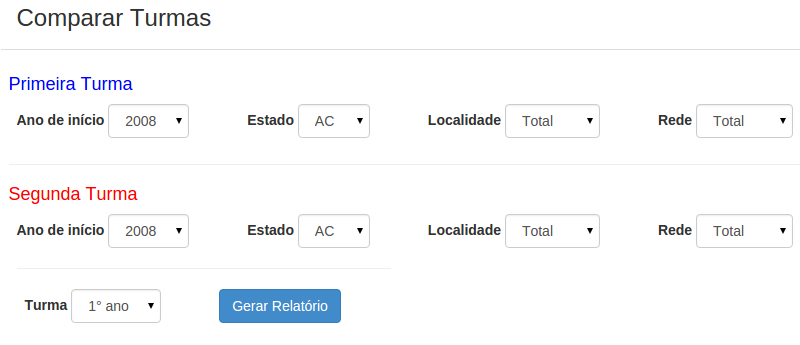
\includegraphics[width=1\textwidth]{imagens/funcionalidadeComparar}
	\caption{Funcionalidade Comparar Turmas}
	\label{img:funcionalidadeComparar}
\end{figure}

Todas as pessoas que utilizaram o sistema apresentaram uma certa dificuldade no momento de selecionar duas turmas. Desse modo, buscamos identificar características que possam ter influenciado nestas dificuldades. Analisando o sistema Enturma e conversando com entrevistados, conseguimos chegar ao resultado da nova interface da comparação de turmas, que será apresentada na figura \ref{img:novaComparacao}, disposta na seção \ref{sub:avalia_o_sistema_enturma_}.

% subsection avalia_o_sistema_enturma_atual (end)

\subsection{Avaliação - Sistema Enturma Modificado} % (fold)
\label{sub:avalia_o_sistema_enturma_}

Após a análise de todos os resultados obtidos com o primeiro questionário, nós decidimos atacar, primeiramente a funcionalidade de Comparação de turmas, a qual chegou a interface apresentada na figura \ref{img:novaComparacao}.

\begin{figure}[H]
	\centering
	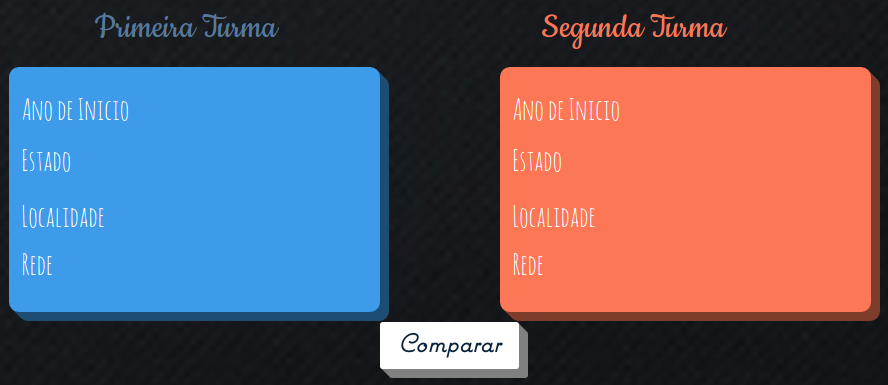
\includegraphics[width=0.9\textwidth]{imagens/novoComparar}
	\caption{Nova Interface da Comparação de Turmas}
	\label{img:novaComparacao}
\end{figure}

Aplicando um novo questionário utilizando esta interface apresentada na figura \ref{img:novaComparacao}, entrevistamos 24 pessoas, sendo 22 homens e 2 mulheres. Esta discrepância ainda se justifica pelo fato da aplicação do questionário ter sido realizada no campus da UnB Gama. Todos os entrevistados possuem conhecimento intermediário ou avançado em computação e utilizam a internet diariamente. 

\begin{table}[H]
	\centering
	\caption{Dados pessoais dos entrevistados do segundo questionário.}
	\label{tab:dadosPessoais2}
	\begin{tabular}{|
		>{\columncolor[HTML]{C0C0C0}}c |c|c|}
		\hline
		\cellcolor[HTML]{C0C0C0}                                                                                                              & \textbf{Homens}                                       & 22                      \\ \cline{2-3} 
		\multirow{-2}{*}{\cellcolor[HTML]{C0C0C0}\textbf{Participantes}}                                                                      & \textbf{Mulheres}                                     & 2                       \\ \hline
		\cellcolor[HTML]{C0C0C0}                                                                                                              & \textbf{18 a 24 anos}                                 & 22                      \\ \cline{2-3} 
		\cellcolor[HTML]{C0C0C0}                                                                                                              & \textbf{25 a 44 anos}                                 & 2                       \\ \cline{2-3} 
		\multirow{-3}{*}{\cellcolor[HTML]{C0C0C0}\textbf{Faixa de Idade}}                                                                     & \textbf{45 a 64 anos}                                 & 0                       \\ \hline
		\cellcolor[HTML]{C0C0C0}                                                                                                              & \textbf{Diária}                                       & 24                      \\ \cline{2-3} 
		\multirow{-2}{*}{\cellcolor[HTML]{C0C0C0}\textbf{\begin{tabular}[c]{@{}c@{}}Frequência com \\ que usa um \\ computador\end{tabular}}} & \textbf{Semanal}                                      & \multicolumn{1}{l|}{0}  \\ \hline
		\cellcolor[HTML]{C0C0C0}                                                                                                              & \textbf{Entre 2 e 5 anos}                             & \multicolumn{1}{l|}{1}  \\ \cline{2-3} 
		\multirow{-2}{*}{\cellcolor[HTML]{C0C0C0}\textbf{\begin{tabular}[c]{@{}c@{}}Possui computador a\\ quanto tempo?\end{tabular}}}        & \textbf{Mais de 5 anos}                               & 23                      \\ \hline
		\cellcolor[HTML]{C0C0C0}                                                                                                              & \textbf{Muito importante}                             & 3                      \\ \cline{2-3} 
		\multirow{-2}{*}{\cellcolor[HTML]{C0C0C0}\textbf{\begin{tabular}[c]{@{}c@{}}Importância da \\ Internet em sua vida\end{tabular}}}     & \multicolumn{1}{l|}{\textbf{Extremamente importante}} & \multicolumn{1}{l|}{21} \\ \hline
	\end{tabular}
\end{table}

Os resultados obtidos neste questionário estão dispostos na tabela \ref{tab:resultados2}. 

\begin{table}[H]
\centering
\caption{Resultados do Segundo Questionário}
\label{tab:resultados2}
	\begin{tabular}{|c|c|}
		\hline
		\rowcolor[HTML]{C0C0C0} 
		\textbf{Visualizar Ranking}                                                                                           & \textbf{Média}        \\ \hline
		Acesso ao Site Enturma                                                                                                & 6,91                  \\ \hline
		Acesso a seção serviços                                                                                               & 6,12                  \\ \hline
		Escolha de uma turma                                                                                                  & 6,2                   \\ \hline
		\begin{tabular}[c]{@{}c@{}}Visualização dos dados\\ obtidos do Ranking\end{tabular}                                   & 6,62                  \\ \hline
		\cellcolor[HTML]{C0C0C0}\textbf{Acompanhamento da Turma}                                                              &                       \\ \hline
		Visualizar relatório de turmas                                                                                        & 7,2                   \\ \hline
		\begin{tabular}[c]{@{}c@{}}Encontrar turma desejada\\ a partir dos filtros\end{tabular}                               & 6,08                  \\ \hline
		Visualizar dados obtidos                                                                                              & 6,33                  \\ \hline
		Limpar dados de pesquisa                                                                                              & 7,2                   \\ \hline
		\cellcolor[HTML]{C0C0C0}\textbf{Comparar Turmas}                                                                      &                       \\ \hline
		Selecionar comparar Turmas                                                                                            & 7,08                  \\ \hline
		\begin{tabular}[c]{@{}c@{}}Selecionar Duas turmas a partir\\ dos seus filtros\end{tabular}                            & 6,5                   \\ \hline
		Visualizar dados obtidos                                                                                              & 7,2                   \\ \hline
		Limpar dados de pesquisa                                                                                              & 7,29                  \\ \hline
		\cellcolor[HTML]{C0C0C0}\textbf{Interface}                                                                            & \multicolumn{1}{l|}{} \\ \hline
		Layout do site                                                                                                        & 6,87                  \\ \hline
		Aspecto visual do site                                                                                                & 6,79                  \\ \hline
		\begin{tabular}[c]{@{}c@{}}Os elementos de informações estão dispostos\\ de forma organizada e racional?\end{tabular} & 6,79                  \\ \hline
	\end{tabular}
\end{table}

Analisando os resultados obtidos nesta tabela é fácil observar a evolução do sistema Enturma após o desenvolvimento deste projeto, na seção \ref{sub:an_lise_dos_resultados_finais} está apresentada a análise dos resultados finais, observando a evolução do sistema Enturma.

% subsection avalia_o_sistema_enturma_ (end)

\subsection{Análise dos Resultados Finais} % (fold)
\label{sub:an_lise_dos_resultados_finais}

% subsection an_lise_dos_resultados_finais (end)